\chapter{Research Questions}
After acknowledging the main research challenges and defining the knowledge gaps that this research will be working on, in this section the main research question is introduced. Also this main question will be broken down into different sub-questions. This strategy has a twofold advantage, on one hand it helps to define small and achievable tasks and it contributes to fill knowledge gaps of different sorts. As seen before, the knowledge domain of this work stands on the intersection of different and diverse fields and consequently, to move forward in the domain of circular economy and urban planning, research is needed in different fronts. For instance, this research will face problems of how to structure and model information of waste flows and explore what metrics could be used to understand progress in terms of circular economy. By first answering smaller and related questions, by the end of the project a bigger picture with an (or partial) answer will emerge. 

\section{Main research question}
Since cities and the network of them that create regions, are crucial to develop a more sustainable local and global future, the effect of different strategies need to be explored. Since 1970 the concept of circular economy has been gained momentum, firstly among the private sector and in the last 5 to 10 years by policy makers. Nowadays, the debate has been also picked up by academia where the concept is being scrutinized. The ideas of circular economy have cross pollinated across a diversity of domains and the urban domain is no exception. Consequently, this creates a variety of questions in the intersection of many knowledge areas. \par
Taking into consideration the research aim and objectives stated above, this research project will be focused on trying to answer the following general research question: \par 

\textbf{\textit{What is the role of spatial configuration in facilitating re-use of waste materials in a city-region?}} % stick to the spatial configuration - and depart from regional planning and institutional political 
% \textbf{\textit{How can spatial urban analysis be integrated into the domain of waste material flow to support planning practices in developing sustainable city-regions?}} \par



\begin{figure}[h!]
    \centering
    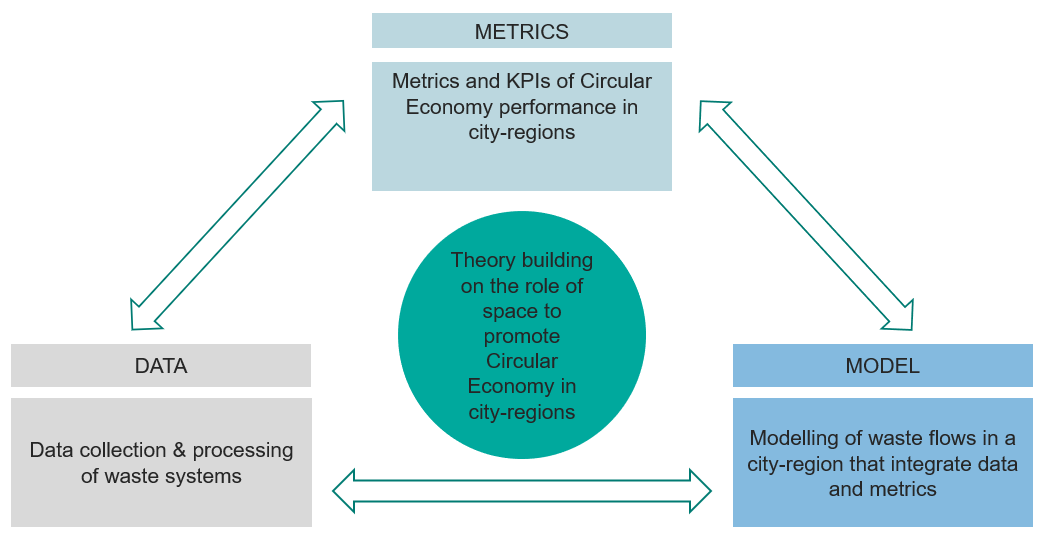
\includegraphics[width=0.8\textwidth]{sections/asset/blocks.PNG}
    \caption{Research components of the project}
    \label{fig:research_bloacks}
\end{figure}



\section{Sub-questions}
In order to bring answers to this main question and contribute to shorten the knowledge gap identified above, the main question is broken down into 9 sub-questions that fall inside 4 different categories of equal importance. As the research project progresses, and specific tasks are accomplished, these sub-questions will be answered. Eventually, after exploring these different sub components an answer to the main question will emerge. \par
Before attempting to answer the main research question,  a set of equally important building blocks are found to be necessary.

\subsubsection{Metrics \& KPIs}
    After reviewing work done in the field of urban metabolism, industrial ecology and or industrial symbiosis, it became clear that most of tools used to analyse the performance of city or region in terms of material use was not incorporating the geographic dimension. The use geographical tools and exploration of how different spatial patterns may (or might not affect) the performance of a system was missing. As a response in order to move forward in the field of circular cities, it is important to answer the following sub questions:\par
    
    \begin{itemize}
        \item \textit{\textbf{RQ1.1: }What KPIs are used to evaluate circular economy in a city-region?}
        \item \textit{\textbf{RQ1.2: }What information is being used to describe and assess circular economy status?}
        \item \textit{\textbf{RQ1.3: }What other metrics can be derived from the spatial configuration of waste flows?}
    \end{itemize}
    
    
\subsubsection{Data models \& simulations}
    Since one big aspect of urban and regional planning is being able to plan for future scenarios or understand how different spatial patterns can influence urban activities, simulations and spatial models are becoming important components of the planning toolkit. For these models to be used by practice they need to be geographic specific. Tools such as Spatial Decision Support Systems (SDSS) and GeoDesign are helping planning agencies to develop better city-regions. Still there is much work to be done in this domain, specifically when it comes to waste materials and how they flow in an a region. On one hand, in these models the location of socioeconomic activities is not taken into consideration, also, in some cases the model used lack the transparency to be used by other researchers or practitioners and lastly, data is still coming from different sources and the field of waste resources has not yet reached a maturity level were there is single data and modelling standard. In transport services, since the development and massive adoption of data standards, there has been a proliferation of different tools and uses for this data. In response to this challenge, the following set of sub-questions will be answered in this project. 
    

    \begin{itemize}
        \item \textit{\textbf{RQ2.1: }How to model the fluxes of waste materials within a city-regions?}
        \item \textit{\textbf{RQ2.2: }Can a general data model hold different types of waste?}
        \item \textit{\textbf{RQ2.3:} How can a spatial model be used to asses the performance in terms of material flow?}
    \end{itemize}


\subsubsection{Data}
    Granular information availability has been growing in the last 5 years. Nowadays, more frequent, more diverse and more precise data is being collected from different sources. Yet, the advancement is not equally distributed across fields. For example, urban transport is one of the most advanced fields were computer science is being applied. The amount of analytical tools and planning applications in transport has shown the importance of collecting and using digital tools to solve urban problems. Yet, when it comes to solid waste, industrial waste or any other sort of by-product, data is being collected at aggregation points. We are capable of knowing how much waste is produced by a country, a region or city  (sometimes) but there are still many data gaps, that does not allow the field to take advantage what digital tools can offer. The lack of data erodes the possibility of creating new tools, and the lack of tools does not create the necessary demand to collect data. 
    
    \begin{itemize}
        \item \textit{\textbf{RQ3.1: }How data of waste flows could be collected to validate the models?}
    \end{itemize}



\subsubsection{Theory}
    Finally, but at the core there are big theoretical questions that could be answered. As the urban digital toolkit continues to expand to waste, by-products or secondary resources, theoretical answers will be able to be answered. As models, data collection and indicators become more precise  and sophisticated, theoretical questions will be answered. By pushing forward the knowledge frontier in the 3 components described above, the possibility of building testable theories in the field of waste materials and urban metabolism will be unlocked.  
    
    \begin{itemize}
        \item \textit{\textbf{RQ4.1: }What are the spatial parameters that contribute to close the loop of resources?}
        \item \textit{\textbf{RQ4.2: }How realistic is to close-loops locally?}
    \end{itemize}



%%%%%%%%%%%%%%%%%%%%%%%%%%%%%%%%%%%%%%%%%%%%%%%%%%%%%%%%%%%%%%%%%%%%%%%%%%%%%%%%%%%%%%%%%%%%%%%%%%%%%%%%%%%%%%%%%%%%%%%%%%%%%%%%%%%%%%%%%%%%%%%%%%%%%%%%%%%%%%%%%%%%%%%%%%%%%%%%%%%%%%%%%%%%%%%%%%%%%%%%%%%%%%%%%%%%%%%%%%%%%%%%%%%%%%%%%%%%%%%%%%%%%%%%%%%%%%%%%%%%%%%%%%%%%%%%%%%%%%%%%%%%%%%%%%%%%%%%%%%%%%%%%%%%%%%%


    % How can the fluxes of waste materials produced in a city-regions be modelled? (as data and model)

    % What are the data requirements to model how resources flow in a city-region?
    
    % Can a general data model be used to hold different types of waste resources?
    
    % What are the spatial parameters that contribute to close the loop of resources?
    
    % Does space needs to be taken into consideration in the KPIs?
    
    % What KPIs can be used to evaluate the degree of circular economy in a city-region?
    
    % How to evaluate the performance of a city-region in terms of closing loops?
    
    % Are these KPIs taking into consideration the spatial parameters of waste flows?
    
    % What other metrics can be derived from the spatial configuration of waste flows?
    
    % What information is being captured in case studies of waste material flow?
    
    %How desegregated is waste resources data published?
    
    % What tools could be used to capture and feed a model of waste fluxes?
    
    % How realistic is to close-loops locally? 
    
    % Can the loop of resources be fully closed %within the city-regions boundaries?
    
    % How is the flow of waste resources in a city-region being assessed and what key performance indicators are calculated in order to evaluate how sustainable waste materials flow in a region?
    
    % How can the exchange of waste materials between industries in a region be spatially modelled? 
    
    % How should waste materials flow in a region in order to achieve an optimal resource usage? 
    
    % How much would it cost to achieve an optimal flow of waste material at a regional level?
    
    % How would a model that captures the flow of waste materials in a region should look like? What are the necessary attributes needed? What can be learnt by reviewing well documented case studies?
    
    % What are the potential uses of such a model? Can this model structure be also used to model the waste at a city level generated by households and managed by a municipality?
    
    % Do conclusions drawn from a-spatial material flow diagrams are still valid if space and the costs of moving residual material are taken into account?  

    % Does waste sorting and collaboration with urban recyclers improve the efficiency of urban solid waste management systems?

    % How to develop a methodology that can quantify and classify waste generated by house holds?

    % How can IoT be incorporated in waste bins to produce an information feed that can be used by to improve the waste management system?
    
    % What is the role of informal waste collectors in the global south? How can their activity be visualised?
    
    % How can information exchanges between generators and pickers could contribute to increase the recycling rates? 